\documentclass[12pt, letterpaper]{article}
\usepackage[utf8]{inputenc}
\usepackage{longtable}
\usepackage{graphicx}
\graphicspath{ {images/} }

\title{Recognition of emotions in speech:\\overview and implementation}
\author{Aydar Musin\\Supervisor: prof. Maxim Talanov}
\date{June 2015, Innopolis University}

\begin{document}

\begin{titlepage}
\maketitle
\end{titlepage}

\begin{abstract}
In this paper will be considered research on recognition of emotions in speech, distinguished their techniques, advantages and disadvantages. Then will be offered own simple implementation of the recognition system.
\end{abstract}

\section{Introduction}

Speech emotion recognition has many application areas. More evident of them: robots and improving the quality of customer service.

If robot has ability to emotional speech generating, it will help him to interact with people better. Because understanding of speech emotion recognition gives understanding how to generate emotional speech. And robots with emotional speech are more people-friendly. Also, speech emotion recognition can improve the robot's decision-making system. Because there are situations when a robot needs to take into account human emotions. %Привести пример!!!!!

Closer to reality application of this system is within an estimation of customer service quality. For example, call-centers have records of conversations. And for operator's work estimation we can identify expressive conversations and analyze them.

There are many research where described dependencies between human emotions and acoustic characteristics. Main differences between them in using different:
\begin{itemize}
	\item Acoustics characteristics
	\item Features
	\item Classification techniques
	\item Recognizable emotions
\end{itemize}

The main goal of this study is to consider these differences and implement own simple solution.
\\
\\
\\
\\

\section{Overview}
\subsection{Acoustic characteristics}
Before we consider a few studies, let's consider some acoustic characteristics:
\begin{itemize}
	\item Pitch or fundamental frequency
	\item Loudness or intensity
	\item Formants
	\item MFCC (Mel-frequency cepstrum coefficients)
\end{itemize}

\subsubsection{Pitch}
Human speech frequency is approximately in the range of 300 to 3400 Hz. The fundamental frequency of speech for male from 85 to 185 Hz, for female from 165 to 255.
\begin{quote}
The fundamental frequency, often referred to simply as the fundamental, is defined as the lowest frequency of a periodic waveform. In terms of a superposition of sinusoids (e.g. Fourier series), the fundamental frequency is the lowest frequency sinusoidal in the sum [http://en.wikipedia.org/wiki/Fundamental\_frequency].
\end{quote}

\subsubsection{Formant and MFCC}
The most frequently in studies used only pitch and loudness. Although formant and MFCC characteristics also useful.
\begin{quote}
Formant is a range of frequencies [of a complex sound] in which there is an absolute or relative maximum in the sound spectrum".[2] In speech science and phonetics, however, a formant is also sometimes used to mean an acoustic resonance[3] of the human vocal tract.[http://en.wikipedia.org/wiki/Formant]
\\
\\
In sound processing, the mel-frequency cepstrum (MFC) is a representation of the short-term power spectrum of a sound, based on a linear cosine transform of a log power spectrum on a nonlinear mel scale of frequency.
\end{quote}


\subsection{Features}
For emotion classifying from acoustic characteristics is necessary extract some features of these characteristics for every emotion. We extract and compute emotion features from training set to use it for classification. And classification is as follows:
\begin{enumerate}
	\item Extract features from processed speech
	\item Compare extracted features with emotion's features
\end{enumerate}

Features can be divided to two types by how to compute and how to compare them:
\begin{itemize}
	\item speaker-dependent
	\item speaker-independent
\end{itemize}

\subsubsection{Speaker-dependent features}
At first, with speaker-dependent features we need a divided training set for every person. And compute features for every person. When classifying we need to compare extracted features with personal features. Advantages of this technique: can be more precisely and much features are not needed. These features based on some average values. For example: average pitch, average intensity, pitch range, intensity range. And they are different for every person. That is why it is not a universal technique because requires statistics keeping for each person. And it is can be applied only in a few cases.
\subsubsection{Speaker-independent features}
Unlike a previous technique here divided training set is not required. But the accuracy of classifying depends on number of speech records and number of speakers represented in the training set. Features based on speech signal dynamics, also some average values. For example, pitch DDS (explanation further), intensity DDS, average phrase duration, etc.


\subsection{Classification}
\begin{center}
		\begin{longtable}{p{2cm}|p{3cm}|p{3cm}|p{3cm}}
		\hline
			Classifier & Description & Advantages & Disadvantages  \\
			 
			\hline
   Binary   Decision Tree & Decision Tree is a stream design drawing like structure in which inward hub talks to check on a quality, every extension talks to deduction of check and every leaf hub talks to class title (choice taken in the wake of registering all traits). A way from root to leaf speaks to arrangement runs the display. In alternative examination a conclusion tree and the almost identified influence journal is utilized as a visual and scientific choice support device, where the usual qualities (or required utility) of arguing options are computed. & Easy implementation, easy explanation of input and output relationship Can handle high dimensional data Easy to interpret for small sized trees The learning and classification steps of induction are simple and fast Accuracy is comparable to other classification techniques for many simple data sets Convertible to simple and easy to understand classification rules & Decision-tree learners can create overcomplex trees that do not generalize the facts and figures well. Decision trees can be unstable because small variations in the facts and figures might outcome in a absolutely different tree being developed. This difficulty is mitigated by using decision trees inside an ensemble. The difficulty of discovering an optimal decision tree is known to be NPcomplete under several facets of optimality and even for easy concepts. Consequently, functional decision-tree learning algorithms are founded on heuristic algorithms such as the greedy algorithm where locally optimal decisions are made at each node. Such algorithms will not assurance to return the globally optimal decision tree. There are concepts that are hard to discover because decision trees do not articulate them effortlessly, such as XOR, parity or multiplexer troubles. conclusion tree learners conceive biased trees if some categories dominate. It is thus suggested to balance the dataset prior to fitting with the conclusion tree\\
			\hline
			Artificial Neural Network & An Artificial Neural mesh (ANN) is a facts and figures organising standard that is inspired by the way biotic anxious structures, for example the cerebrum, process facts and figures. The key constituent of this ideal model is the innovative structure of the facts and figures handling structure. It is made out of countless interconnected changing components (neurones) employed as one to tackle specific issues. ANNs, for demonstration persons, study by illustration. An ANN is designed for a specific provision, for demonstration design acknowledgement or information characterization, through a revising method. revising in living structures includes acclimations to the synaptic associations that exist between the neurones. This is accurate of ANNs besides & They can both about any convoluted conclusion supplied that enough nodes are utilised. Neural systems are rather easy to implement (you do not need a good linear algebra solver as for examples for SVNs). Neural networks often exhibit patterns alike to those exhibited by humans. although this is more of interest in cognitive sciences than for functional examples & Long preparing time The VC measurement of neural systems is indistinct. This is extremely critical when you need to think about how exceptional an answer could be. Neural systems can't be retrained. Provided that you include information later, this is just about difficult to add to an existing system. Taking care of time arrangement information in neural systems is an exceptionally confounded point.\\
			\hline
			Naïve Bayes classifier&The Naive Bayes Classifier procedure is reliant upon the purported Bayesian hypothesis and is particularly suited when the dimensionality of the inputs is high. Notwithstanding its effortlessness, Naive Bayes can frequently outflank more refined grouping strategies&Fast to train (single scan). Fast to classify Not sensitive to irrelevant features Handles real and discrete data Handles streaming data well&Assumes independence of features
			\hline
			\caption{Classification methods comparison}
			\label{tab:ClassificationMethodsComparison}
		\end{longtable}
	
\end{center}

\subsection{Recognizable emotions}
Accuracy of recognition depends not only on extracted features and used classifier, also it depends on recognized emotions. It is caused by that some emotions are very similar. And to improve classifying similar emotions is necessary improve features extraction and classifier. More emotions- less accuracy. That is why it is a trade-off between recognizable emotions and accuracy.
\begin{figure}[t]
	\centering
		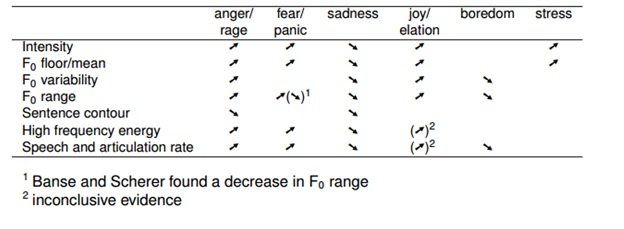
\includegraphics[scale=0.8]{emotion-table-example}
	\caption{Sound characteristics for emotions [1]}
	\label{fig:emotion-table-example}
\end{figure}

For example, at the Figure 1 showed some features of emotions. And we can see that some emotions very similar(anger-joy,sadness-boredom). Although number of emotions is not so large. But with increasing number of emotions, also increases intersections between emotions on features. So it's important to define emotions which is needed for particular task

\section{Implementation}
\subsection{The goal in general}
The main goal is to implement simple recognition system. The program should have ability to recognize emotions from sound file or microphone. Also, it should be resistant to interference and noise. Implementation will be carried out using C\# programming language.

Implementation can be divided to four steps:
\begin{enumerate}
	\item Extracting sound characteristics from sound file or microphone
	\item Speech splitting to phrases or words
	\item Feature extraction and analyzing
	\item Classification
\end{enumerate}

\begin{figure}
	\centering
		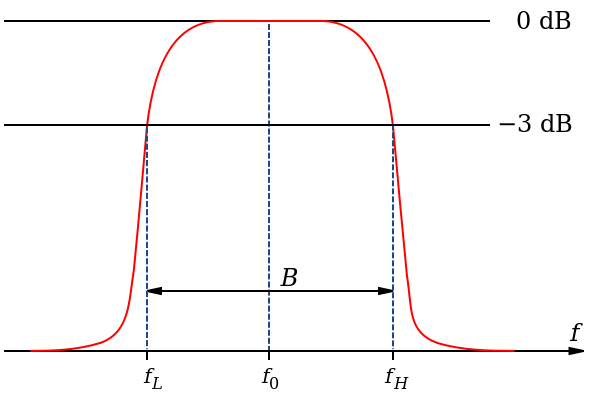
\includegraphics[scale=0.7]{images/pass-band-filter.png}
	\caption{Pass-band filter}
	\label{fig:pass-band-filter}
\end{figure}

\subsubsection{Extracting sound characteristics}

At first, is important to note that we need only voice characteristics and to avoid wrong results sound should be filtered. At first, is important to note that we need only voice characteristics and to avoid wrong results sound should be filtered. Filtering is important not only because is needed correct voice characteristics, also because it provides ability distinguish voiced and unvoiced intervals of speech. 
\\

To retrieve sound characteristics using C\# one can use these libraries:
\begin{itemize}
	\item NAudio (http://naudio.codeplex.com)
	\item Bass Audio library (http://naudio.codeplex.com)
\end{itemize}

But these libraries provide only sound signal receiving from file or microphone. And to get sound characteristic, for example pitch, we have to implement also Fast Fourier Transform function. Also, we have to implement filtering function. For example, simplest filtering can be implemented as pass-band filter. 

Pass-band filter just establish range of signal values, and if signal values go beyond they will be ignored.(Figure 2)
\\
There is also software package which fits our goals - PRAAT. It is often used for speech analyzing and contains all needed functions:
\begin{itemize}
	\item Get fundamental frequency (pitch)
	\item Get loudness
	\item Get spectrogram
	\item Get formant
	\item Filtering function
\end{itemize}

That are functions that we will use, but package contains a lot more functions. And for using all function it has own script language. 

For filtering in the package is using \textit{Remove noise} function. Which consists of pass-band filter and special functions for white noise removing.

Eventually, using PRAAT we will get from sound file these characteristics:
\begin{itemize}
	\item Pitch, or F0
	\item Loudness, or intensity
	\item Formant (F1, F2, F3)
	\item Center of gravity of spectrogram
\end{itemize}
Graphics for these characteristics represented in the Figure 3. We can see that there are intervals where values are equal to zero. It is the result of filter working. When pitch (F0) goes beyond human speech frequency range, all values are assigned to zero.
\begin{figure}
	\centering
		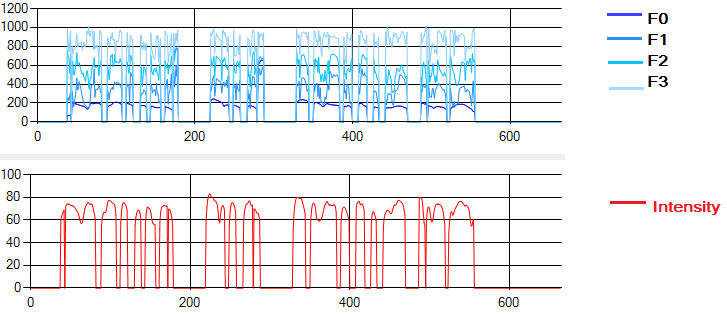
\includegraphics[scale=0.8]{images/sound-characteristics.png}
	\caption{Extracted sound characteristics}
	\label{fig:sound-characteristics}
\end{figure}

\subsubsection{Dividing speech to phrases}

Because when people are speaking, they express emotions by changing some characteristics of phrases or words. And for accurate recognition is needed to divide speech to phrases and analyze them separately.

It is worth noting, that precise dividing is impossible without filtering. That is why successfulness of  this step very strong related with previous step. In output from previous step we get set of characteristics where silence intervals marked as zeros. So, algorithm can be as follows: 

 \begin{itemize}
	 \item Until zero value, collect phrase values
		\item After zero value, ends with this phrase and go to the next
 \end{itemize}

But problem with this in that a few zeros can appear in the middle of the phrase. And to solve this problem we should set the minimum length of zeros between phrases. At the Figure 3 is shown speech divided to phrases, and within phrase exist intervals of zeros but they are slight. 

So after two steps in the output is received set of sound characteristics and phrase pointers. It is now necessary to extract features for classification.
\begin{figure}
	\centering
		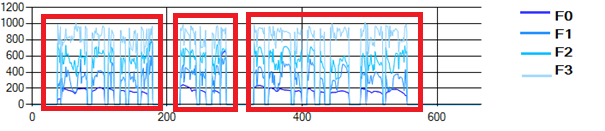
\includegraphics[scale=1]{images/phrases.png}
	\caption{Speech divided to phrases}
	\label{fig:phrases}
\end{figure}
\\
\\
\\
\\
\\
\\

\subsection{Features extraction}

\begin{table}

\begin{tabular}{|p{2.2in}|p{2.2in}|} 
\hline
\multirow{Pitch (F0) }& Variance \\ \cline{2-2}
													& Range \\ \cline{2-2} 
													& DDS \\ \hline 
Formant 1 (F1) & DDS \\ \hline 
Formant 2 (F2) & DDS \\ \hline 
Formant 2 (F3) & DDS \\ \hline 
\multirow{Loudness (Intensity) } & Variance \\ \cline{2-2}
																		& Range \\ \cline{2-2}
																		& DDS \\ \hline 
\multirow{Time} & mean phrase duration \\ \cline{2-2} 
 & mean silence duration \\ \hline 
Spectrogramm & Center of gravity (centroid) \\ \hline 
\end{tabular}
	\caption{Using features}
	\label{Using features}
\end{table}
\emph{Variance.} It can be calculated by standard deviation of set:
\begin{center}
\[V=\sqrt{
\sum_{i=0}^{n}{
               (x_i-\overline{x})^2
               }
}
\]
 where  $\overline{x}$ is average of set
\end{center}
\\
\\
\emph{Range} It is difference between maximum and minimum
\\
\\
\emph{DDS (Difference-Distance-Slope)} This feature is calculating for each phrase( Example in the Figure 5) 
\begin{itemize}
	\item Find local $maximum$ and $minimum$ elements for phrase
	\item $difference=maximum-minimum$
	\item $distance=maximum_{position}-minimum_{position}$
\end{itemize}

\begin{figure}
	\centering
		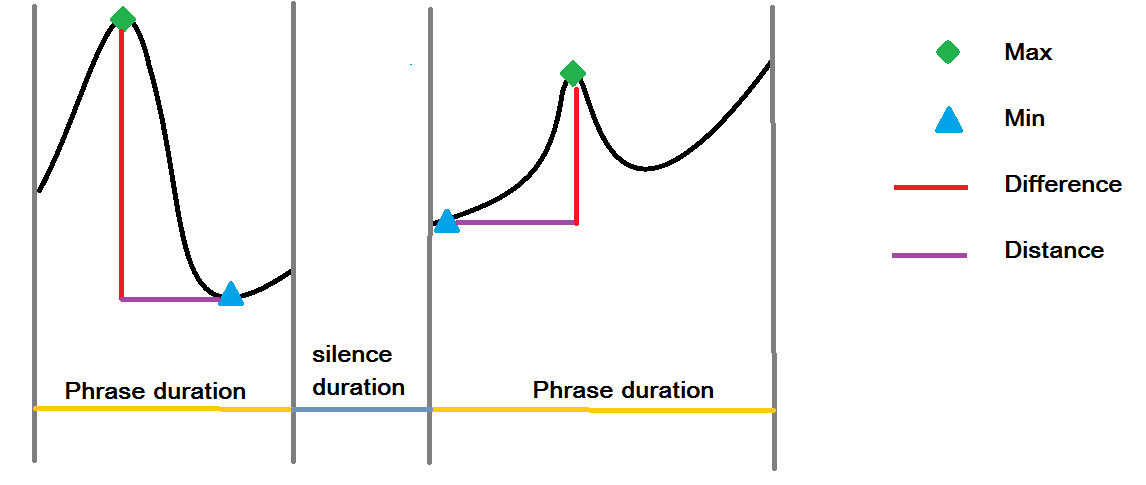
\includegraphics[scale=0.5]{images/dds.png}
	\caption{DDS}
	\label{fig:phrases}
\end{figure}
Phrase duration and silence duration are calculating by phrase pointers. Also, center of gravity of spectrogram for all speech provides PRAAT. 
\subsection{Features from training data set}

As a training data set we use EmoDB[http://emodb.bilderbar.info]. It is emotional database which consist of speech records of 10 different actors. For classification we use only four basic emotions: anger, happiness,sadness,neutral. And from EmoDB we use 107 records with these emotions and different texts. Results of features extraction represented in Table 3.
\begin{table}[h]
	\centering
		\begin{tabular}{l|l|l|l|l|}
			\hline
				Feature/Emotion& anger&	happy	&sadness	&neutral\\ \hline
PitchDff&	137,08	&211,55	&67,32	&64,63\\ \hline 
PitchDis&	-6	&-10,125&	-19,33&	-8\\ \hline
IntDif&	22,22&	22,92&	19,63&	18,76\\ \hline
IntDis	&6,44	&-5,83&	-7,41&	-3,2\\ \hline
F1Dif&	239,44&	228,16&	210,52&	193,49\\ \hline
F1Dis&	-1,71	&-5,87&	-9&	-1,66\\ \hline
F2dif	&349,82&	318,56&	340,58&	299,02\\ \hline
F2Dis&	-1,42&	-3,15&	-2,32	&0,66\\ \hline
F3Dif&	355,51&	359,38&	449,35&	425,46\\ \hline
F3Dis&	-0,4	&-2,28&	-0,33&	2,6\\ \hline
PitchRange&	465,16&	406,37&	150,065&	457,2\\ \hline
IntRange&	31,36&	28,95&	28,865&	27,61\\ \hline
PitchVariance&	7253,96&	10823,92&	1737,46&	6720,77\\ \hline
IntVariance	&46,19&	41,20&	35,10	&36,24\\ \hline
PhraseDuration&	28,9&	38,16&	39,58	&24,66\\ \hline
SilenceDuration	&5,2	&4,45	&5,375&	5,4\\ \hline
Centroid&	580,3	&519,54&	359,08&	350,02\\ \hline
 \hline
		\end{tabular}
	\caption{Extracted features from training data set. Dif-Difference, Dis-Distance, Int-Intensity}
	\label{tab:ExtractedFeaturesFromTrainingDataSet}
\end{table}

\subsection{Classification}
So we have got some feature values for each emotion, and is needed to build classifier using them. There are impossible to set strict confines for features values for each emotion. Because emotion feature value is median for all analyzed speech records and some values very different from this value. In addition, some feature values are very similar and it's difficult divide them to four classes. But often among these 4 values exist two high and two low values. It caused by fact that some emotion very similar with some features, but they have some distinct features.
For example: angry-happy, sadness-neutral. It can be seen on the Table 3, most of the features of angry and happiness are similar, there are some features which distinct for them. For example, phrase duration is lower for angry.

That is why was decided to use fuzzy sets for classifying each feature to two classes: \emph{high} and \emph{low}. Because classification to 2 classes will be more precise. And fuzzy sets allow to set intersection between them.
\end{document}
